\section{\it QuickSort}

\begin{frame}[fragile]{Motivação}

    \begin{itemize}
        \item Embora o \textit{MergeSort} seja um algoritmo que atinja a limite
            inferior $O(N\log N)$ para algoritmos de ordenação baseados em
            comparações, ele demanda uma memória adicional $O(N)$, não sendo portando
            um algoritmo \textit{in-place}

        \item A ideia do \textit{QuickSort} é aproveitar a ideia da divisão do vetor em
            subvetores menores, como é feito no \textit{MergeSort}

        \item Contudo, a ideia é que o algoritmo seja \textit{in-place}

        \item Assim, a divisão do vetor não será posicional, mas sim baseada no valor de um
            elemento escolhido arbitrariamente, denominado pivô

        \item O pivô permite um rearranjo dos elementos usando a própria memória do vetor,
            tornando o algoritmo \textit{in-place}

        \item Embora o \textit{QuickSort} tenha complexidade média $O(N\log N)$, no pior caso
            ele pode se degenerar para $O(N^2)$
    \end{itemize}

\end{frame}

\begin{frame}[fragile]{Pivoteamento}

    \begin{itemize}
        \item Pivoteamento é o processo de reposicionamento dos elementos do vetor
            de acordo com o valor $x$ do elemento pivô que ocupa o índice $p$

        \item Ao final do pivoteamento, todos elementos com valores menores que $x$ estarão
            à esquerda do pivô, e os demais à direita

        \item O pivô já estará na posição correta em relação ao ordenamento global, de modo que
            o  \textit{QuickSort} pode prosseguir recursivamente nas duas partes separadas
            pelo pivô

        \item Para simplificar a rotina, no início do pivoteamento o pivô troca de posição
            com o primeiro elemento do vetor

        \item Ao final, o pivô se move para a posição adequada e esta posição é retornada

        \item Para evitar o pior caso, a escolha do pivô deve ser aleatória entre todos 
            os índices possíveis
    \end{itemize}

\end{frame}

\begin{frame}[fragile]{Visualização da rotina de pivoteamento}

    \begin{figure}
        \centering

        \begin{tikzpicture}
            \draw (0, 5) grid (9, 6);

            \draw[->] (3.5,6.5) node[anchor=south] { $p$ } -- (3.5,6.25);
            \draw[opacity=0,->] (1.5,4.5) node[anchor=north] { $i$ } -- (1.5,4.75);
            \draw[opacity=0,->] (1.5,6.5) node[anchor=south] { $j$ } -- (1.5,6.25);
            \draw[opacity=0,->] (9.5,6.5) node[anchor=south] { $j$ } -- (9.5,6.25);

            \node at (0.5, 5.5) { \textcolor{black}{$89$} };
            \node at (1.5, 5.5) { \textcolor{black}{$60$} };
            \node at (2.5, 5.5) { \textcolor{black}{$12$} };
            \node at (3.5, 5.5) { \textcolor{black}{$45$} };
            \node at (4.5, 5.5) { \textcolor{black}{$37$} };
            \node at (5.5, 5.5) { \textcolor{black}{$52$} };
            \node at (6.5, 5.5) { \textcolor{black}{$33$} };
            \node at (7.5, 5.5) { \textcolor{black}{$97$} };
            \node at (8.5, 5.5) { \textcolor{black}{$20$} };

        \end{tikzpicture}

    \end{figure}

\end{frame}

\begin{frame}[fragile]{Visualização da rotina de pivoteamento}

    \begin{figure}
        \centering

        \begin{tikzpicture}
            \draw (0, 5) grid (9, 6);

            \draw[->] (3.5,6.5) node[anchor=south] { $p$ } -- (3.5,6.25);
            \draw[opacity=0,->] (1.5,4.5) node[anchor=north] { $i$ } -- (1.5,4.75);
            \draw[opacity=0,->] (1.5,6.5) node[anchor=south] { $j$ } -- (1.5,6.25);
            \draw[opacity=0,->] (9.5,6.5) node[anchor=south] { $j$ } -- (9.5,6.25);

            \node at (0.5, 5.5) { \textcolor{green!60!black}{$89$} };
            \node at (1.5, 5.5) { \textcolor{black}{$60$} };
            \node at (2.5, 5.5) { \textcolor{black}{$12$} };
            \node at (3.5, 5.5) { \textcolor{blue}{$45$} };
            \node at (4.5, 5.5) { \textcolor{black}{$37$} };
            \node at (5.5, 5.5) { \textcolor{black}{$52$} };
            \node at (6.5, 5.5) { \textcolor{black}{$33$} };
            \node at (7.5, 5.5) { \textcolor{black}{$97$} };
            \node at (8.5, 5.5) { \textcolor{black}{$20$} };

        \end{tikzpicture}

    \end{figure}

\end{frame}

\begin{frame}[fragile]{Visualização da rotina de pivoteamento}

    \begin{figure}
        \centering

        \begin{tikzpicture}
            \draw (0, 5) grid (9, 6);

            \draw[->] (0.5,6.5) node[anchor=south] { $p$ } -- (0.5,6.25);
            \draw[opacity=0,->] (1.5,4.5) node[anchor=north] { $i$ } -- (1.5,4.75);
            \draw[opacity=0,->] (1.5,6.5) node[anchor=south] { $j$ } -- (1.5,6.25);
            \draw[opacity=0,->] (9.5,6.5) node[anchor=south] { $j$ } -- (9.5,6.25);

            \node at (0.5, 5.5) { \textcolor{blue}{$45$} };
            \node at (1.5, 5.5) { \textcolor{black}{$60$} };
            \node at (2.5, 5.5) { \textcolor{black}{$12$} };
            \node at (3.5, 5.5) { \textcolor{green!60!black}{$89$} };
            \node at (4.5, 5.5) { \textcolor{black}{$37$} };
            \node at (5.5, 5.5) { \textcolor{black}{$52$} };
            \node at (6.5, 5.5) { \textcolor{black}{$33$} };
            \node at (7.5, 5.5) { \textcolor{black}{$97$} };
            \node at (8.5, 5.5) { \textcolor{black}{$20$} };

        \end{tikzpicture}

    \end{figure}

\end{frame}

\begin{frame}[fragile]{Visualização da rotina de pivoteamento}

    \begin{figure}
        \centering

        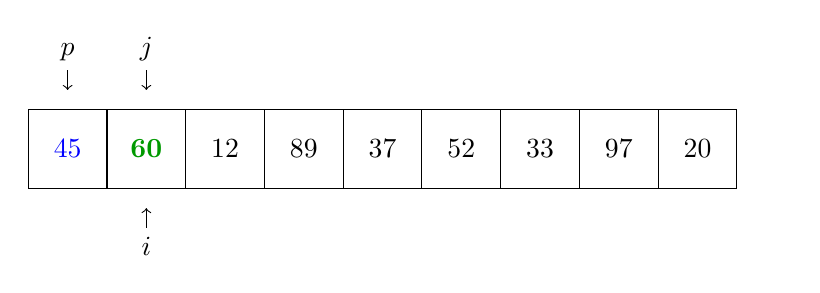
\begin{tikzpicture}
            \draw (0, 5) grid (9, 6);

            \draw[->] (0.5,6.5) node[anchor=south] { $p$ } -- (0.5,6.25);
            \draw[opacity=1,->] (1.5,4.5) node[anchor=north] { $i$ } -- (1.5,4.75);
            \draw[opacity=1,->] (1.5,6.5) node[anchor=south] { $j$ } -- (1.5,6.25);
            \draw[opacity=0,->] (9.5,6.5) node[anchor=south] { $j$ } -- (9.5,6.25);

            \node at (0.5, 5.5) { \textcolor{blue}{$45$} };
            \node at (1.5, 5.5) { \textcolor{green!60!black}{$\mathbf{60}$} };
            \node at (2.5, 5.5) { \textcolor{black}{$12$} };
            \node at (3.5, 5.5) { \textcolor{black}{$89$} };
            \node at (4.5, 5.5) { \textcolor{black}{$37$} };
            \node at (5.5, 5.5) { \textcolor{black}{$52$} };
            \node at (6.5, 5.5) { \textcolor{black}{$33$} };
            \node at (7.5, 5.5) { \textcolor{black}{$97$} };
            \node at (8.5, 5.5) { \textcolor{black}{$20$} };

        \end{tikzpicture}

    \end{figure}

\end{frame}

\begin{frame}[fragile]{Visualização da rotina de pivoteamento}

    \begin{figure}
        \centering

        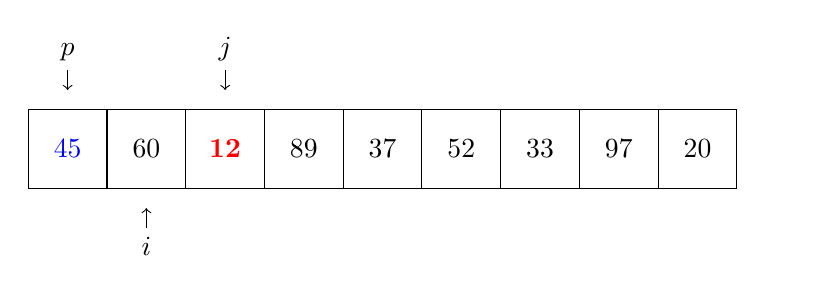
\begin{tikzpicture}
            \draw (0, 5) grid (9, 6);

            \draw[->] (0.5,6.5) node[anchor=south] { $p$ } -- (0.5,6.25);
            \draw[opacity=1,->] (1.5,4.5) node[anchor=north] { $i$ } -- (1.5,4.75);
            \draw[opacity=1,->] (2.5,6.5) node[anchor=south] { $j$ } -- (2.5,6.25);
            \draw[opacity=0,->] (9.5,6.5) node[anchor=south] { $j$ } -- (9.5,6.25);

            \node at (0.5, 5.5) { \textcolor{blue}{$45$} };
            \node at (1.5, 5.5) { \textcolor{black}{$60$} };
            \node at (2.5, 5.5) { \textcolor{red}{$\mathbf{12}$} };
            \node at (3.5, 5.5) { \textcolor{black}{$89$} };
            \node at (4.5, 5.5) { \textcolor{black}{$37$} };
            \node at (5.5, 5.5) { \textcolor{black}{$52$} };
            \node at (6.5, 5.5) { \textcolor{black}{$33$} };
            \node at (7.5, 5.5) { \textcolor{black}{$97$} };
            \node at (8.5, 5.5) { \textcolor{black}{$20$} };

        \end{tikzpicture}

    \end{figure}

\end{frame}

\begin{frame}[fragile]{Visualização da rotina de pivoteamento}

    \begin{figure}
        \centering

        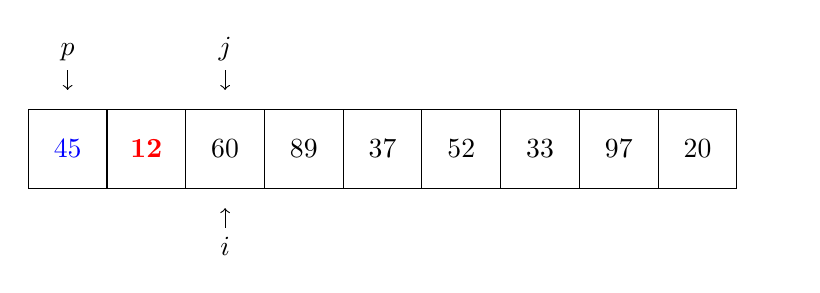
\begin{tikzpicture}
            \draw (0, 5) grid (9, 6);

            \draw[->] (0.5,6.5) node[anchor=south] { $p$ } -- (0.5,6.25);
            \draw[opacity=1,->] (2.5,4.5) node[anchor=north] { $i$ } -- (2.5,4.75);
            \draw[opacity=1,->] (2.5,6.5) node[anchor=south] { $j$ } -- (2.5,6.25);
            \draw[opacity=0,->] (9.5,6.5) node[anchor=south] { $j$ } -- (9.5,6.25);

            \node at (0.5, 5.5) { \textcolor{blue}{$45$} };
            \node at (2.5, 5.5) { \textcolor{black}{$60$} };
            \node at (1.5, 5.5) { \textcolor{red}{$\mathbf{12}$} };
            \node at (3.5, 5.5) { \textcolor{black}{$89$} };
            \node at (4.5, 5.5) { \textcolor{black}{$37$} };
            \node at (5.5, 5.5) { \textcolor{black}{$52$} };
            \node at (6.5, 5.5) { \textcolor{black}{$33$} };
            \node at (7.5, 5.5) { \textcolor{black}{$97$} };
            \node at (8.5, 5.5) { \textcolor{black}{$20$} };

        \end{tikzpicture}

    \end{figure}

\end{frame}

\begin{frame}[fragile]{Visualização da rotina de pivoteamento}

    \begin{figure}
        \centering

        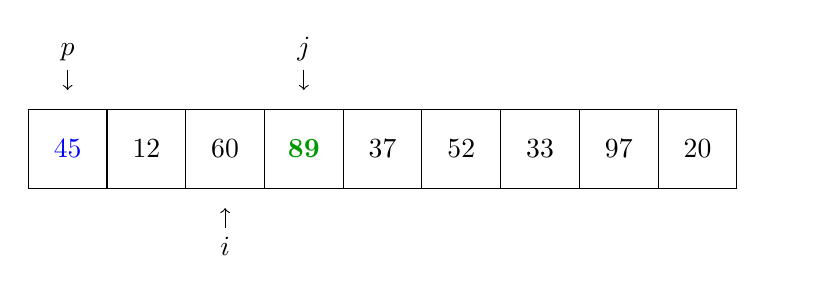
\begin{tikzpicture}
            \draw (0, 5) grid (9, 6);

            \draw[->] (0.5,6.5) node[anchor=south] { $p$ } -- (0.5,6.25);
            \draw[opacity=1,->] (2.5,4.5) node[anchor=north] { $i$ } -- (2.5,4.75);
            \draw[opacity=1,->] (3.5,6.5) node[anchor=south] { $j$ } -- (3.5,6.25);
            \draw[opacity=0,->] (9.5,6.5) node[anchor=south] { $j$ } -- (9.5,6.25);

            \node at (0.5, 5.5) { \textcolor{blue}{$45$} };
            \node at (1.5, 5.5) { \textcolor{black}{$12$} };
            \node at (2.5, 5.5) { \textcolor{black}{$60$} };
            \node at (3.5, 5.5) { \textcolor{green!60!black}{$\mathbf{89}$} };
            \node at (4.5, 5.5) { \textcolor{black}{$37$} };
            \node at (5.5, 5.5) { \textcolor{black}{$52$} };
            \node at (6.5, 5.5) { \textcolor{black}{$33$} };
            \node at (7.5, 5.5) { \textcolor{black}{$97$} };
            \node at (8.5, 5.5) { \textcolor{black}{$20$} };

        \end{tikzpicture}

    \end{figure}

\end{frame}

\begin{frame}[fragile]{Visualização da rotina de pivoteamento}

    \begin{figure}
        \centering

        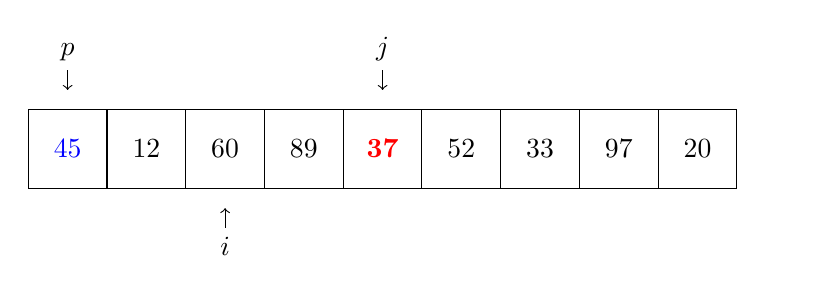
\begin{tikzpicture}
            \draw (0, 5) grid (9, 6);

            \draw[->] (0.5,6.5) node[anchor=south] { $p$ } -- (0.5,6.25);
            \draw[opacity=1,->] (2.5,4.5) node[anchor=north] { $i$ } -- (2.5,4.75);
            \draw[opacity=1,->] (4.5,6.5) node[anchor=south] { $j$ } -- (4.5,6.25);
            \draw[opacity=0,->] (9.5,6.5) node[anchor=south] { $j$ } -- (9.5,6.25);

            \node at (0.5, 5.5) { \textcolor{blue}{$45$} };
            \node at (1.5, 5.5) { \textcolor{black}{$12$} };
            \node at (2.5, 5.5) { \textcolor{black}{$60$} };
            \node at (3.5, 5.5) { \textcolor{black}{$89$} };
            \node at (4.5, 5.5) { \textcolor{red}{$\mathbf{37}$} };
            \node at (5.5, 5.5) { \textcolor{black}{$52$} };
            \node at (6.5, 5.5) { \textcolor{black}{$33$} };
            \node at (7.5, 5.5) { \textcolor{black}{$97$} };
            \node at (8.5, 5.5) { \textcolor{black}{$20$} };

        \end{tikzpicture}

    \end{figure}

\end{frame}

\begin{frame}[fragile]{Visualização da rotina de pivoteamento}

    \begin{figure}
        \centering

        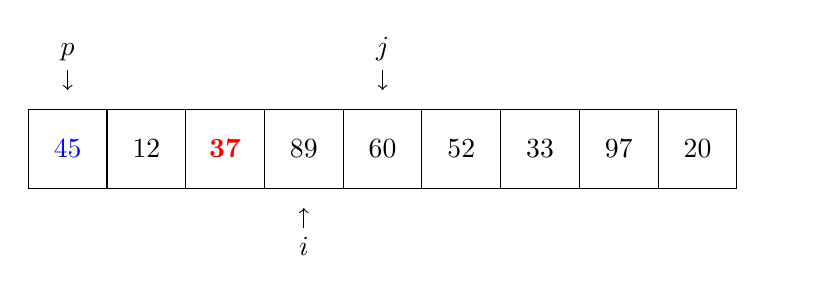
\begin{tikzpicture}
            \draw (0, 5) grid (9, 6);

            \draw[->] (0.5,6.5) node[anchor=south] { $p$ } -- (0.5,6.25);
            \draw[opacity=1,->] (3.5,4.5) node[anchor=north] { $i$ } -- (3.5,4.75);
            \draw[opacity=1,->] (4.5,6.5) node[anchor=south] { $j$ } -- (4.5,6.25);
            \draw[opacity=0,->] (9.5,6.5) node[anchor=south] { $j$ } -- (9.5,6.25);

            \node at (0.5, 5.5) { \textcolor{blue}{$45$} };
            \node at (1.5, 5.5) { \textcolor{black}{$12$} };
            \node at (2.5, 5.5) { \textcolor{red}{$\mathbf{37}$} };
            \node at (3.5, 5.5) { \textcolor{black}{$89$} };
            \node at (4.5, 5.5) { \textcolor{black}{$60$} };
            \node at (5.5, 5.5) { \textcolor{black}{$52$} };
            \node at (6.5, 5.5) { \textcolor{black}{$33$} };
            \node at (7.5, 5.5) { \textcolor{black}{$97$} };
            \node at (8.5, 5.5) { \textcolor{black}{$20$} };

        \end{tikzpicture}

    \end{figure}

\end{frame}

\begin{frame}[fragile]{Visualização da rotina de pivoteamento}

    \begin{figure}
        \centering

        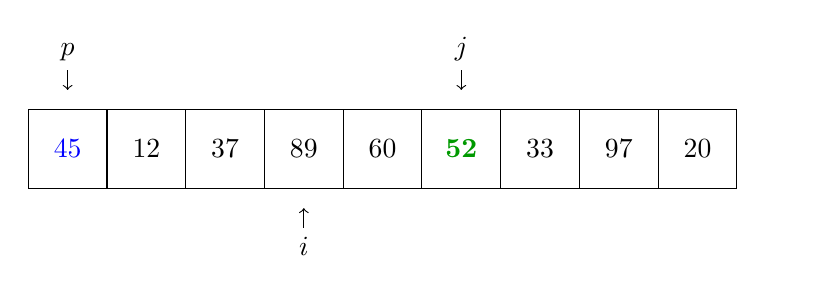
\begin{tikzpicture}
            \draw (0, 5) grid (9, 6);

            \draw[->] (0.5,6.5) node[anchor=south] { $p$ } -- (0.5,6.25);
            \draw[opacity=1,->] (3.5,4.5) node[anchor=north] { $i$ } -- (3.5,4.75);
            \draw[opacity=1,->] (5.5,6.5) node[anchor=south] { $j$ } -- (5.5,6.25);
            \draw[opacity=0,->] (9.5,6.5) node[anchor=south] { $j$ } -- (9.5,6.25);

            \node at (0.5, 5.5) { \textcolor{blue}{$45$} };
            \node at (1.5, 5.5) { \textcolor{black}{$12$} };
            \node at (2.5, 5.5) { \textcolor{black}{$37$} };
            \node at (3.5, 5.5) { \textcolor{black}{$89$} };
            \node at (4.5, 5.5) { \textcolor{black}{$60$} };
            \node at (5.5, 5.5) { \textcolor{green!60!black}{$\mathbf{52}$} };
            \node at (6.5, 5.5) { \textcolor{black}{$33$} };
            \node at (7.5, 5.5) { \textcolor{black}{$97$} };
            \node at (8.5, 5.5) { \textcolor{black}{$20$} };

        \end{tikzpicture}

    \end{figure}

\end{frame}

\begin{frame}[fragile]{Visualização da rotina de pivoteamento}

    \begin{figure}
        \centering

        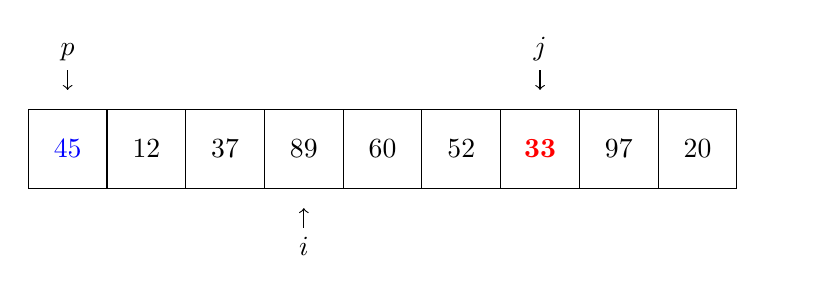
\begin{tikzpicture}
            \draw (0, 5) grid (9, 6);

            \draw[->] (0.5,6.5) node[anchor=south] { $p$ } -- (0.5,6.25);
            \draw[opacity=1,->] (3.5,4.5) node[anchor=north] { $i$ } -- (3.5,4.75);
            \draw[opacity=1,->] (6.5,6.5) node[anchor=south] { $j$ } -- (6.5,6.25);
            \draw[opacity=0,->] (9.5,6.5) node[anchor=south] { $j$ } -- (9.5,6.25);

            \node at (0.5, 5.5) { \textcolor{blue}{$45$} };
            \node at (1.5, 5.5) { \textcolor{black}{$12$} };
            \node at (2.5, 5.5) { \textcolor{black}{$37$} };
            \node at (3.5, 5.5) { \textcolor{black}{$89$} };
            \node at (4.5, 5.5) { \textcolor{black}{$60$} };
            \node at (5.5, 5.5) { \textcolor{black}{$52$} };
            \node at (6.5, 5.5) { \textcolor{red}{$\mathbf{33}$} };
            \node at (7.5, 5.5) { \textcolor{black}{$97$} };
            \node at (8.5, 5.5) { \textcolor{black}{$20$} };

        \end{tikzpicture}

    \end{figure}

\end{frame}

\begin{frame}[fragile]{Visualização da rotina de pivoteamento}

    \begin{figure}
        \centering

        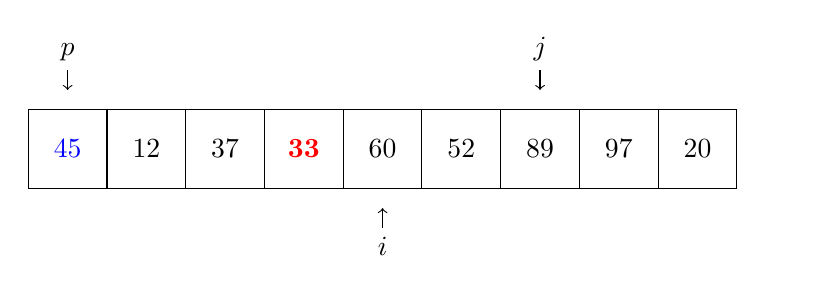
\begin{tikzpicture}
            \draw (0, 5) grid (9, 6);

            \draw[->] (0.5,6.5) node[anchor=south] { $p$ } -- (0.5,6.25);
            \draw[opacity=1,->] (4.5,4.5) node[anchor=north] { $i$ } -- (4.5,4.75);
            \draw[opacity=1,->] (6.5,6.5) node[anchor=south] { $j$ } -- (6.5,6.25);
            \draw[opacity=0,->] (9.5,6.5) node[anchor=south] { $j$ } -- (9.5,6.25);

            \node at (0.5, 5.5) { \textcolor{blue}{$45$} };
            \node at (1.5, 5.5) { \textcolor{black}{$12$} };
            \node at (2.5, 5.5) { \textcolor{black}{$37$} };
            \node at (3.5, 5.5) { \textcolor{red}{$\mathbf{33}$} };
            \node at (4.5, 5.5) { \textcolor{black}{$60$} };
            \node at (5.5, 5.5) { \textcolor{black}{$52$} };
            \node at (6.5, 5.5) { \textcolor{black}{$89$} };
            \node at (7.5, 5.5) { \textcolor{black}{$97$} };
            \node at (8.5, 5.5) { \textcolor{black}{$20$} };

        \end{tikzpicture}

    \end{figure}

\end{frame}

\begin{frame}[fragile]{Visualização da rotina de pivoteamento}

    \begin{figure}
        \centering

        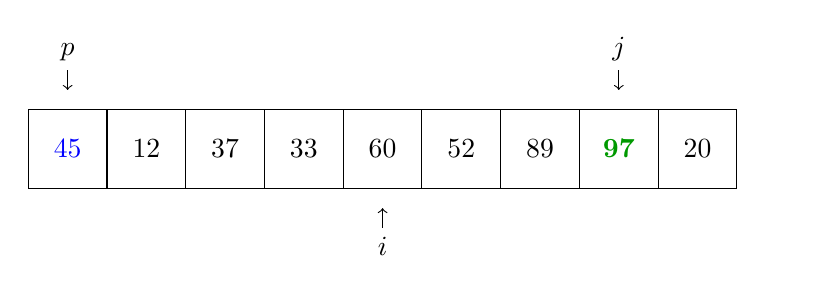
\begin{tikzpicture}
            \draw (0, 5) grid (9, 6);

            \draw[->] (0.5,6.5) node[anchor=south] { $p$ } -- (0.5,6.25);
            \draw[opacity=1,->] (4.5,4.5) node[anchor=north] { $i$ } -- (4.5,4.75);
            \draw[opacity=1,->] (7.5,6.5) node[anchor=south] { $j$ } -- (7.5,6.25);
            \draw[opacity=0,->] (9.5,6.5) node[anchor=south] { $j$ } -- (9.5,6.25);

            \node at (0.5, 5.5) { \textcolor{blue}{$45$} };
            \node at (1.5, 5.5) { \textcolor{black}{$12$} };
            \node at (2.5, 5.5) { \textcolor{black}{$37$} };
            \node at (3.5, 5.5) { \textcolor{black}{$33$} };
            \node at (4.5, 5.5) { \textcolor{black}{$60$} };
            \node at (5.5, 5.5) { \textcolor{black}{$52$} };
            \node at (6.5, 5.5) { \textcolor{black}{$89$} };
            \node at (7.5, 5.5) { \textcolor{green!60!black}{$\mathbf{97}$} };
            \node at (8.5, 5.5) { \textcolor{black}{$20$} };

        \end{tikzpicture}

    \end{figure}

\end{frame}

\begin{frame}[fragile]{Visualização da rotina de pivoteamento}

    \begin{figure}
        \centering

        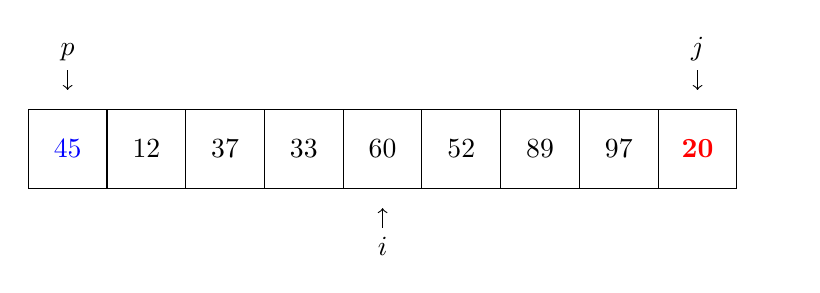
\begin{tikzpicture}
            \draw (0, 5) grid (9, 6);

            \draw[->] (0.5,6.5) node[anchor=south] { $p$ } -- (0.5,6.25);
            \draw[opacity=1,->] (4.5,4.5) node[anchor=north] { $i$ } -- (4.5,4.75);
            \draw[opacity=1,->] (8.5,6.5) node[anchor=south] { $j$ } -- (8.5,6.25);
            \draw[opacity=0,->] (9.5,6.5) node[anchor=south] { $j$ } -- (9.5,6.25);

            \node at (0.5, 5.5) { \textcolor{blue}{$45$} };
            \node at (1.5, 5.5) { \textcolor{black}{$12$} };
            \node at (2.5, 5.5) { \textcolor{black}{$37$} };
            \node at (3.5, 5.5) { \textcolor{black}{$33$} };
            \node at (4.5, 5.5) { \textcolor{black}{$60$} };
            \node at (5.5, 5.5) { \textcolor{black}{$52$} };
            \node at (6.5, 5.5) { \textcolor{black}{$89$} };
            \node at (7.5, 5.5) { \textcolor{black}{$97$} };
            \node at (8.5, 5.5) { \textcolor{red}{$\mathbf{20}$} };

        \end{tikzpicture}

    \end{figure}

\end{frame}

\begin{frame}[fragile]{Visualização da rotina de pivoteamento}

    \begin{figure}
        \centering

        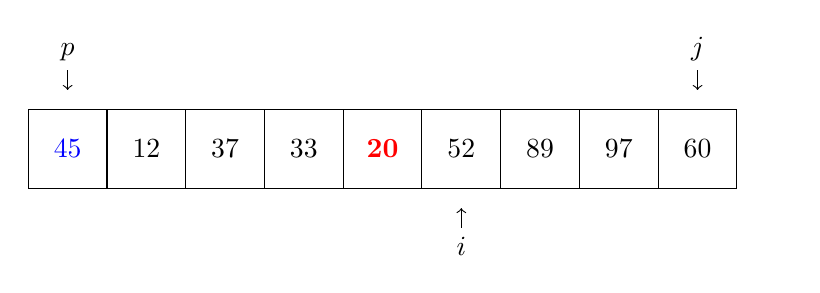
\begin{tikzpicture}
            \draw (0, 5) grid (9, 6);

            \draw[->] (0.5,6.5) node[anchor=south] { $p$ } -- (0.5,6.25);
            \draw[opacity=1,->] (5.5,4.5) node[anchor=north] { $i$ } -- (5.5,4.75);
            \draw[opacity=1,->] (8.5,6.5) node[anchor=south] { $j$ } -- (8.5,6.25);
            \draw[opacity=0,->] (9.5,6.5) node[anchor=south] { $j$ } -- (9.5,6.25);

            \node at (0.5, 5.5) { \textcolor{blue}{$45$} };
            \node at (1.5, 5.5) { \textcolor{black}{$12$} };
            \node at (2.5, 5.5) { \textcolor{black}{$37$} };
            \node at (3.5, 5.5) { \textcolor{black}{$33$} };
            \node at (4.5, 5.5) { \textcolor{red}{$\mathbf{20}$} };
            \node at (5.5, 5.5) { \textcolor{black}{$52$} };
            \node at (6.5, 5.5) { \textcolor{black}{$89$} };
            \node at (7.5, 5.5) { \textcolor{black}{$97$} };
            \node at (8.5, 5.5) { \textcolor{black}{$60$} };

        \end{tikzpicture}

    \end{figure}

\end{frame}

\begin{frame}[fragile]{Visualização da rotina de pivoteamento}

    \begin{figure}
        \centering

        \begin{tikzpicture}
            \draw (0, 5) grid (9, 6);

            \draw[->] (0.5,6.5) node[anchor=south] { $p$ } -- (0.5,6.25);
            \draw[opacity=1,->] (5.5,4.5) node[anchor=north] { $i$ } -- (5.5,4.75);
            \draw[opacity=1,->] (9.5,6.5) node[anchor=south] { $j$ } -- (9.5,6.25);

            \node at (0.5, 5.5) { \textcolor{blue}{$45$} };
            \node at (1.5, 5.5) { \textcolor{black}{$12$} };
            \node at (2.5, 5.5) { \textcolor{black}{$37$} };
            \node at (3.5, 5.5) { \textcolor{black}{$33$} };
            \node at (4.5, 5.5) { \textcolor{black}{$20$} };
            \node at (5.5, 5.5) { \textcolor{black}{$52$} };
            \node at (6.5, 5.5) { \textcolor{black}{$89$} };
            \node at (7.5, 5.5) { \textcolor{black}{$97$} };
            \node at (8.5, 5.5) { \textcolor{black}{$60$} };

        \end{tikzpicture}

    \end{figure}

\end{frame}


\begin{frame}[fragile]{Visualização da rotina de pivoteamento}

    \begin{figure}
        \centering

        \begin{tikzpicture}
            \draw (0, 5) grid (9, 6);

            \draw[->] (0.5,6.5) node[anchor=south] { $p$ } -- (0.5,6.25);
            \draw[opacity=1,->] (5.5,4.5) node[anchor=north] { $i$ } -- (5.5,4.75);
            \draw[opacity=1,->] (9.5,6.5) node[anchor=south] { $j$ } -- (9.5,6.25);

            \node at (0.5, 5.5) { \textcolor{blue}{$45$} };
            \node at (1.5, 5.5) { \textcolor{black}{$12$} };
            \node at (2.5, 5.5) { \textcolor{black}{$37$} };
            \node at (3.5, 5.5) { \textcolor{black}{$33$} };
            \node at (4.5, 5.5) { \textcolor{green!60!black}{$20$} };
            \node at (5.5, 5.5) { \textcolor{black}{$52$} };
            \node at (6.5, 5.5) { \textcolor{black}{$89$} };
            \node at (7.5, 5.5) { \textcolor{black}{$97$} };
            \node at (8.5, 5.5) { \textcolor{black}{$60$} };

        \end{tikzpicture}

    \end{figure}

\end{frame}

\begin{frame}[fragile]{Visualização da rotina de pivoteamento}

    \begin{figure}
        \centering

        \begin{tikzpicture}
            \draw (0, 5) grid (9, 6);

            \draw[->] (4.5,6.5) node[anchor=south] { $p$ } -- (4.5,6.25);
            \draw[opacity=1,->] (5.5,4.5) node[anchor=north] { $i$ } -- (5.5,4.75);
            \draw[opacity=1,->] (9.5,6.5) node[anchor=south] { $j$ } -- (9.5,6.25);

            \node at (0.5, 5.5) { \textcolor{green!60!black}{$20$} };
            \node at (1.5, 5.5) { \textcolor{black}{$12$} };
            \node at (2.5, 5.5) { \textcolor{black}{$37$} };
            \node at (3.5, 5.5) { \textcolor{black}{$33$} };
            \node at (4.5, 5.5) { \textcolor{blue}{$45$} };
            \node at (5.5, 5.5) { \textcolor{black}{$52$} };
            \node at (6.5, 5.5) { \textcolor{black}{$89$} };
            \node at (7.5, 5.5) { \textcolor{black}{$97$} };
            \node at (8.5, 5.5) { \textcolor{black}{$60$} };

        \end{tikzpicture}

    \end{figure}

\end{frame}


\begin{frame}[fragile]{Implementação da rotina de pivoteamento}
    \inputsnippet{cpp}{5}{25}{codes/quicksort.cpp}
\end{frame}


\begin{frame}[fragile]{Visualização do {\it quicksort}}

    \begin{figure}
        \centering

        \begin{tikzpicture}
            \draw (0, 5) grid (9, 6);
            \draw[opacity=0] (0, 3) grid (9, 4);
            \draw[opacity=0] (0, 1) grid (9, 2);
            \draw[opacity=0] (0, -1) grid (9, 0);

            \draw[opacity=0] (0, -2) rectangle (1,-1);
            \draw[opacity=0,->] (3.5,4.5) node[anchor=north] { $p$ } -- (3.5,4.9);
            \draw[opacity=0,->] (3.5,-1.5) node[anchor=north] { $p$ } -- (3.5,-1.1);

            \node at (0.5, 5.5) { \textcolor{black}{$89$} };
            \node at (1.5, 5.5) { \textcolor{black}{$60$} };
            \node at (2.5, 5.5) { \textcolor{black}{$12$} };
            \node at (3.5, 5.5) { \textcolor{black}{$45$} };
            \node at (4.5, 5.5) { \textcolor{black}{$37$} };
            \node at (5.5, 5.5) { \textcolor{black}{$52$} };
            \node at (6.5, 5.5) { \textcolor{black}{$33$} };
            \node at (7.5, 5.5) { \textcolor{black}{$97$} };
            \node at (8.5, 5.5) { \textcolor{black}{$20$} };

        \end{tikzpicture}

    \end{figure}

\end{frame}

\begin{frame}[fragile]{Visualização do {\it quicksort}}

    \begin{figure}
        \centering

        \begin{tikzpicture}
            \draw (0, 5) grid (9, 6);
            \draw[opacity=0] (0, 3) grid (9, 4);
            \draw[opacity=0] (0, 1) grid (9, 2);
            \draw[opacity=0] (0, -1) grid (9, 0);

            \draw[opacity=0] (0, -2) rectangle (1,-1);
            \draw[opacity=1,->] (3.5,4.5) node[anchor=north] { $p$ } -- (3.5,4.9);
            \draw[opacity=0,->] (3.5,-1.5) node[anchor=north] { $p$ } -- (3.5,-1.1);

            \node at (0.5, 5.5) { \textcolor{black}{$89$} };
            \node at (1.5, 5.5) { \textcolor{black}{$60$} };
            \node at (2.5, 5.5) { \textcolor{black}{$12$} };
            \node at (3.5, 5.5) { \textcolor{black}{$45$} };
            \node at (4.5, 5.5) { \textcolor{black}{$37$} };
            \node at (5.5, 5.5) { \textcolor{black}{$52$} };
            \node at (6.5, 5.5) { \textcolor{black}{$33$} };
            \node at (7.5, 5.5) { \textcolor{black}{$97$} };
            \node at (8.5, 5.5) { \textcolor{black}{$20$} };

        \end{tikzpicture}

    \end{figure}

\end{frame}

\begin{frame}[fragile]{Visualização do {\it quicksort}}

    \begin{figure}
        \centering

        \begin{tikzpicture}
            \draw (0, 5) grid (9, 6);
            \draw[opacity=1] (0, 3) grid (9, 4);
            \draw[opacity=0] (0, 1) grid (9, 2);
            \draw[opacity=0] (0, -1) grid (9, 0);

            \draw[opacity=0] (0, -2) rectangle (1,-1);
            \draw[opacity=1,->] (3.5,4.5) node[anchor=north] { $p$ } -- (3.5,4.9);
            \draw[opacity=0,->] (3.5,-1.5) node[anchor=north] { $p$ } -- (3.5,-1.1);

            \node at (0.5, 5.5) { \textcolor{black}{$89$} };
            \node at (1.5, 5.5) { \textcolor{black}{$60$} };
            \node at (2.5, 5.5) { \textcolor{black}{$12$} };
            \node at (3.5, 5.5) { \textcolor{black}{$45$} };
            \node at (4.5, 5.5) { \textcolor{black}{$37$} };
            \node at (5.5, 5.5) { \textcolor{black}{$52$} };
            \node at (6.5, 5.5) { \textcolor{black}{$33$} };
            \node at (7.5, 5.5) { \textcolor{black}{$97$} };
            \node at (8.5, 5.5) { \textcolor{black}{$20$} };

            \node at (0.5, 3.5) { \textcolor{black}{$20$} };
            \node at (1.5, 3.5) { \textcolor{black}{$12$} };
            \node at (2.5, 3.5) { \textcolor{black}{$37$} };
            \node at (3.5, 3.5) { \textcolor{black}{$33$} };
            \node at (4.5, 3.5) { \textcolor{blue}{$\mathbf{45}$} };
            \node at (5.5, 3.5) { \textcolor{black}{$52$} };
            \node at (6.5, 3.5) { \textcolor{black}{$89$} };
            \node at (7.5, 3.5) { \textcolor{black}{$97$} };
            \node at (8.5, 3.5) { \textcolor{black}{$60$} };

        \end{tikzpicture}

    \end{figure}

\end{frame}

\begin{frame}[fragile]{Visualização do {\it quicksort}}

    \begin{figure}
        \centering

        \begin{tikzpicture}
            \draw (0, 5) grid (9, 6);
            \draw[opacity=1] (0, 3) grid (9, 4);
            \draw[opacity=0] (0, 1) grid (9, 2);
            \draw[opacity=0] (0, -1) grid (9, 0);

            \draw[opacity=0] (0, -2) rectangle (1,-1);
            \draw[opacity=1,->] (0.5,2.5) node[anchor=north] { $p$ } -- (0.5,2.9);
            \draw[opacity=1,->] (6.5,2.5) node[anchor=north] { $p$ } -- (6.5,2.9);

            \node at (0.5, 5.5) { \textcolor{black}{$89$} };
            \node at (1.5, 5.5) { \textcolor{black}{$60$} };
            \node at (2.5, 5.5) { \textcolor{black}{$12$} };
            \node at (3.5, 5.5) { \textcolor{black}{$45$} };
            \node at (4.5, 5.5) { \textcolor{black}{$37$} };
            \node at (5.5, 5.5) { \textcolor{black}{$52$} };
            \node at (6.5, 5.5) { \textcolor{black}{$33$} };
            \node at (7.5, 5.5) { \textcolor{black}{$97$} };
            \node at (8.5, 5.5) { \textcolor{black}{$20$} };

            \node at (0.5, 3.5) { \textcolor{black}{$20$} };
            \node at (1.5, 3.5) { \textcolor{black}{$12$} };
            \node at (2.5, 3.5) { \textcolor{black}{$37$} };
            \node at (3.5, 3.5) { \textcolor{black}{$33$} };
            \node at (4.5, 3.5) { \textcolor{blue}{$45$} };
            \node at (5.5, 3.5) { \textcolor{black}{$52$} };
            \node at (6.5, 3.5) { \textcolor{black}{$89$} };
            \node at (7.5, 3.5) { \textcolor{black}{$97$} };
            \node at (8.5, 3.5) { \textcolor{black}{$60$} };

        \end{tikzpicture}

    \end{figure}

\end{frame}

\begin{frame}[fragile]{Visualização do {\it quicksort}}

    \begin{figure}
        \centering

        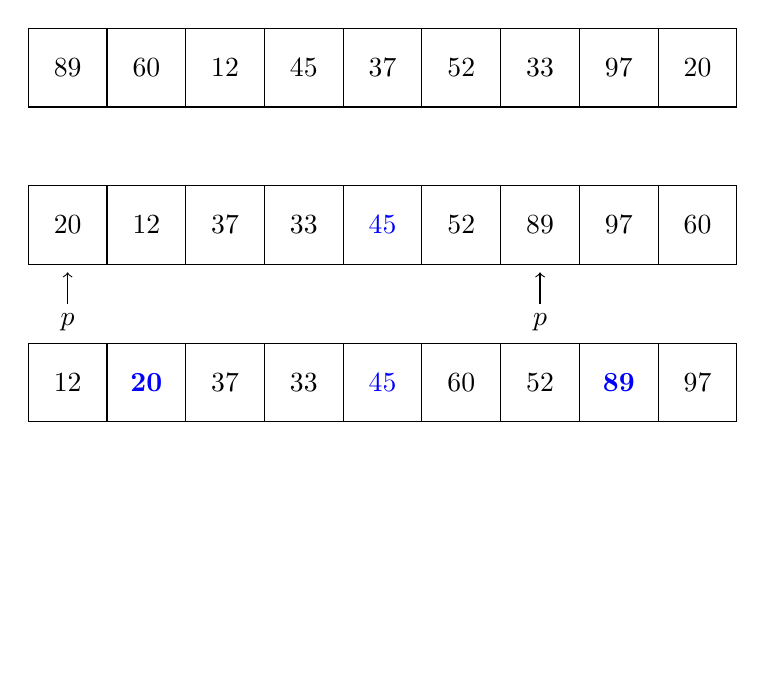
\begin{tikzpicture}
            \draw (0, 5) grid (9, 6);
            \draw[opacity=1] (0, 3) grid (9, 4);
            \draw[opacity=1] (0, 1) grid (9, 2);
            \draw[opacity=0] (0, -1) grid (9, 0);

            \draw[opacity=0] (0, -2) rectangle (1,-1);
            \draw[opacity=1,->] (0.5,2.5) node[anchor=north] { $p$ } -- (0.5,2.9);
            \draw[opacity=1,->] (6.5,2.5) node[anchor=north] { $p$ } -- (6.5,2.9);

            \node at (0.5, 5.5) { \textcolor{black}{$89$} };
            \node at (1.5, 5.5) { \textcolor{black}{$60$} };
            \node at (2.5, 5.5) { \textcolor{black}{$12$} };
            \node at (3.5, 5.5) { \textcolor{black}{$45$} };
            \node at (4.5, 5.5) { \textcolor{black}{$37$} };
            \node at (5.5, 5.5) { \textcolor{black}{$52$} };
            \node at (6.5, 5.5) { \textcolor{black}{$33$} };
            \node at (7.5, 5.5) { \textcolor{black}{$97$} };
            \node at (8.5, 5.5) { \textcolor{black}{$20$} };

            \node at (0.5, 3.5) { \textcolor{black}{$20$} };
            \node at (1.5, 3.5) { \textcolor{black}{$12$} };
            \node at (2.5, 3.5) { \textcolor{black}{$37$} };
            \node at (3.5, 3.5) { \textcolor{black}{$33$} };
            \node at (4.5, 3.5) { \textcolor{blue}{$45$} };
            \node at (5.5, 3.5) { \textcolor{black}{$52$} };
            \node at (6.5, 3.5) { \textcolor{black}{$89$} };
            \node at (7.5, 3.5) { \textcolor{black}{$97$} };
            \node at (8.5, 3.5) { \textcolor{black}{$60$} };

            \node at (0.5, 1.5) { \textcolor{black}{$12$} };
            \node at (1.5, 1.5) { \textcolor{blue}{$\mathbf{20}$} };
            \node at (2.5, 1.5) { \textcolor{black}{$37$} };
            \node at (3.5, 1.5) { \textcolor{black}{$33$} };
            \node at (4.5, 1.5) { \textcolor{blue}{$45$} };
            \node at (5.5, 1.5) { \textcolor{black}{$60$} };
            \node at (6.5, 1.5) { \textcolor{black}{$52$} };
            \node at (7.5, 1.5) { \textcolor{blue}{$\mathbf{89}$} };
            \node at (8.5, 1.5) { \textcolor{black}{$97$} };

        \end{tikzpicture}

    \end{figure}

\end{frame}

\begin{frame}[fragile]{Visualização do {\it quicksort}}

    \begin{figure}
        \centering

        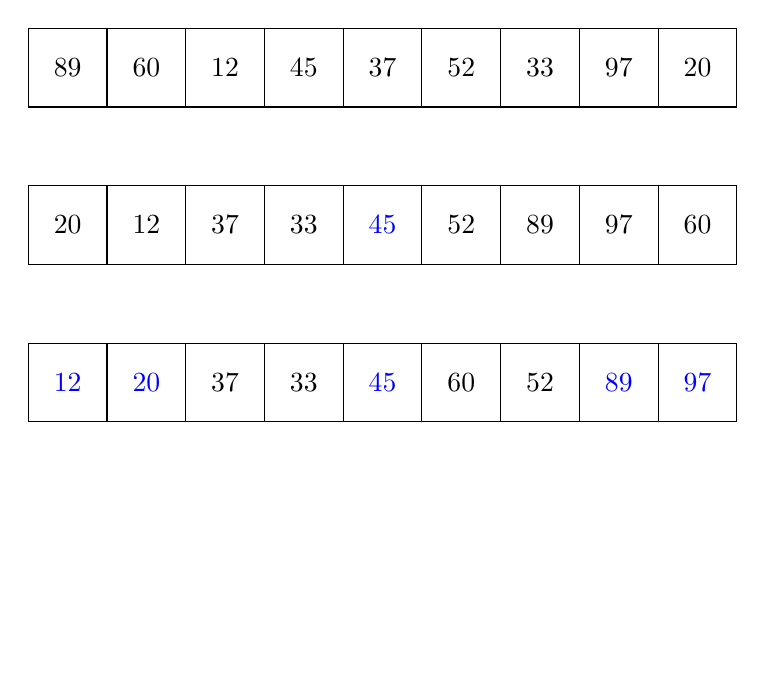
\begin{tikzpicture}
            \draw (0, 5) grid (9, 6);
            \draw[opacity=1] (0, 3) grid (9, 4);
            \draw[opacity=1] (0, 1) grid (9, 2);
            \draw[opacity=0] (0, -1) grid (9, 0);

            \draw[opacity=0] (0, -2) rectangle (1,-1);
            \draw[opacity=0,->] (0.5,2.5) node[anchor=north] { $p$ } -- (0.5,2.9);
            \draw[opacity=0,->] (6.5,2.5) node[anchor=north] { $p$ } -- (6.5,2.9);

            \node at (0.5, 5.5) { \textcolor{black}{$89$} };
            \node at (1.5, 5.5) { \textcolor{black}{$60$} };
            \node at (2.5, 5.5) { \textcolor{black}{$12$} };
            \node at (3.5, 5.5) { \textcolor{black}{$45$} };
            \node at (4.5, 5.5) { \textcolor{black}{$37$} };
            \node at (5.5, 5.5) { \textcolor{black}{$52$} };
            \node at (6.5, 5.5) { \textcolor{black}{$33$} };
            \node at (7.5, 5.5) { \textcolor{black}{$97$} };
            \node at (8.5, 5.5) { \textcolor{black}{$20$} };

            \node at (0.5, 3.5) { \textcolor{black}{$20$} };
            \node at (1.5, 3.5) { \textcolor{black}{$12$} };
            \node at (2.5, 3.5) { \textcolor{black}{$37$} };
            \node at (3.5, 3.5) { \textcolor{black}{$33$} };
            \node at (4.5, 3.5) { \textcolor{blue}{$45$} };
            \node at (5.5, 3.5) { \textcolor{black}{$52$} };
            \node at (6.5, 3.5) { \textcolor{black}{$89$} };
            \node at (7.5, 3.5) { \textcolor{black}{$97$} };
            \node at (8.5, 3.5) { \textcolor{black}{$60$} };

            \node at (0.5, 1.5) { \textcolor{blue}{$12$} };
            \node at (1.5, 1.5) { \textcolor{blue}{$20$} };
            \node at (2.5, 1.5) { \textcolor{black}{$37$} };
            \node at (3.5, 1.5) { \textcolor{black}{$33$} };
            \node at (4.5, 1.5) { \textcolor{blue}{$45$} };
            \node at (5.5, 1.5) { \textcolor{black}{$60$} };
            \node at (6.5, 1.5) { \textcolor{black}{$52$} };
            \node at (7.5, 1.5) { \textcolor{blue}{$89$} };
            \node at (8.5, 1.5) { \textcolor{blue}{$97$} };

        \end{tikzpicture}

    \end{figure}

\end{frame}

\begin{frame}[fragile]{Visualização do {\it quicksort}}

    \begin{figure}
        \centering

        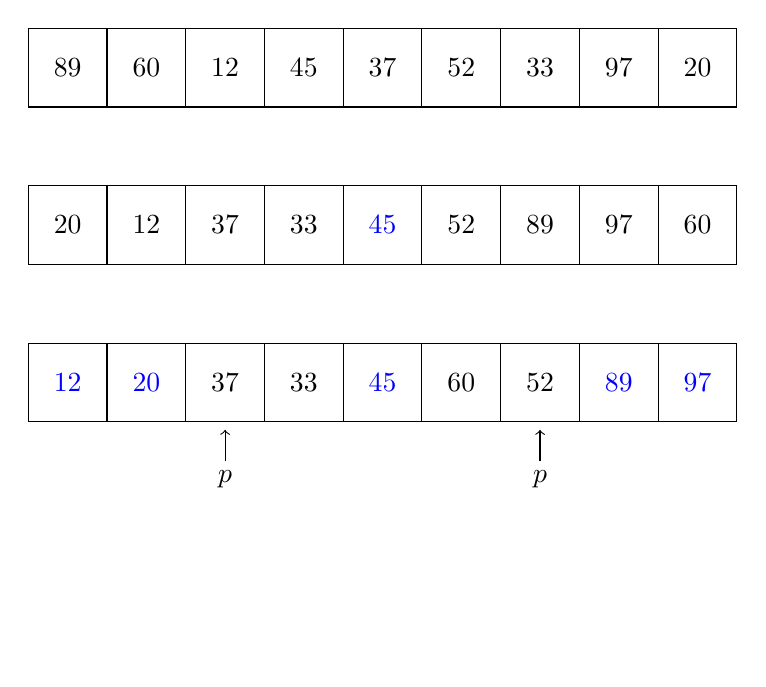
\begin{tikzpicture}
            \draw (0, 5) grid (9, 6);
            \draw[opacity=1] (0, 3) grid (9, 4);
            \draw[opacity=1] (0, 1) grid (9, 2);
            \draw[opacity=0] (0, -1) grid (9, 0);

            \draw[opacity=0] (0, -2) rectangle (1,-1);
            \draw[opacity=1,->] (2.5,0.5) node[anchor=north] { $p$ } -- (2.5,0.9);
            \draw[opacity=1,->] (6.5,0.5) node[anchor=north] { $p$ } -- (6.5,0.9);

            \node at (0.5, 5.5) { \textcolor{black}{$89$} };
            \node at (1.5, 5.5) { \textcolor{black}{$60$} };
            \node at (2.5, 5.5) { \textcolor{black}{$12$} };
            \node at (3.5, 5.5) { \textcolor{black}{$45$} };
            \node at (4.5, 5.5) { \textcolor{black}{$37$} };
            \node at (5.5, 5.5) { \textcolor{black}{$52$} };
            \node at (6.5, 5.5) { \textcolor{black}{$33$} };
            \node at (7.5, 5.5) { \textcolor{black}{$97$} };
            \node at (8.5, 5.5) { \textcolor{black}{$20$} };

            \node at (0.5, 3.5) { \textcolor{black}{$20$} };
            \node at (1.5, 3.5) { \textcolor{black}{$12$} };
            \node at (2.5, 3.5) { \textcolor{black}{$37$} };
            \node at (3.5, 3.5) { \textcolor{black}{$33$} };
            \node at (4.5, 3.5) { \textcolor{blue}{$45$} };
            \node at (5.5, 3.5) { \textcolor{black}{$52$} };
            \node at (6.5, 3.5) { \textcolor{black}{$89$} };
            \node at (7.5, 3.5) { \textcolor{black}{$97$} };
            \node at (8.5, 3.5) { \textcolor{black}{$60$} };

            \node at (0.5, 1.5) { \textcolor{blue}{$12$} };
            \node at (1.5, 1.5) { \textcolor{blue}{$20$} };
            \node at (2.5, 1.5) { \textcolor{black}{$37$} };
            \node at (3.5, 1.5) { \textcolor{black}{$33$} };
            \node at (4.5, 1.5) { \textcolor{blue}{$45$} };
            \node at (5.5, 1.5) { \textcolor{black}{$60$} };
            \node at (6.5, 1.5) { \textcolor{black}{$52$} };
            \node at (7.5, 1.5) { \textcolor{blue}{$89$} };
            \node at (8.5, 1.5) { \textcolor{blue}{$97$} };

        \end{tikzpicture}

    \end{figure}

\end{frame}

\begin{frame}[fragile]{Visualização do {\it quicksort}}

    \begin{figure}
        \centering

        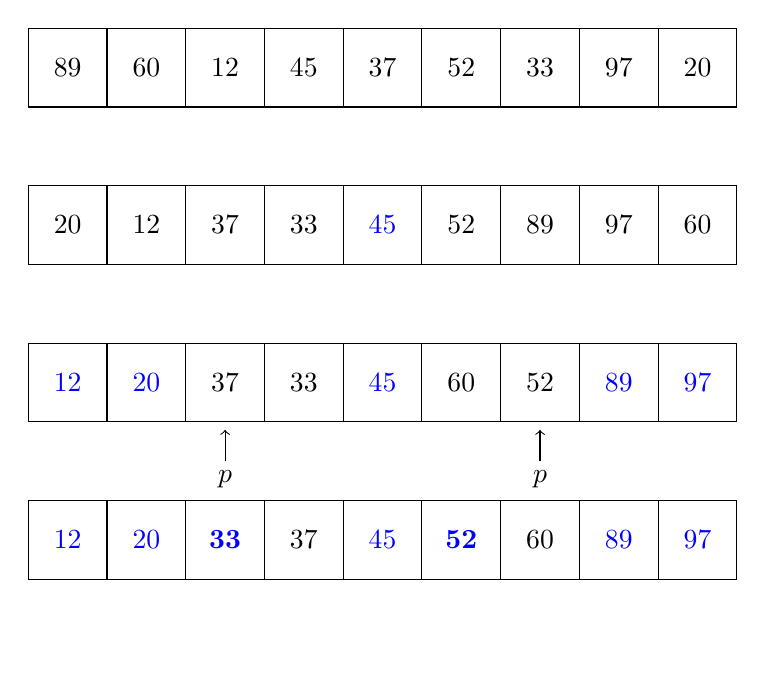
\begin{tikzpicture}
            \draw (0, 5) grid (9, 6);
            \draw[opacity=1] (0, 3) grid (9, 4);
            \draw[opacity=1] (0, 1) grid (9, 2);
            \draw[opacity=1] (0, -1) grid (9, 0);

            \draw[opacity=0] (0, -2) rectangle (1,-1);
            \draw[opacity=1,->] (2.5,0.5) node[anchor=north] { $p$ } -- (2.5,0.9);
            \draw[opacity=1,->] (6.5,0.5) node[anchor=north] { $p$ } -- (6.5,0.9);

            \node at (0.5, 5.5) { \textcolor{black}{$89$} };
            \node at (1.5, 5.5) { \textcolor{black}{$60$} };
            \node at (2.5, 5.5) { \textcolor{black}{$12$} };
            \node at (3.5, 5.5) { \textcolor{black}{$45$} };
            \node at (4.5, 5.5) { \textcolor{black}{$37$} };
            \node at (5.5, 5.5) { \textcolor{black}{$52$} };
            \node at (6.5, 5.5) { \textcolor{black}{$33$} };
            \node at (7.5, 5.5) { \textcolor{black}{$97$} };
            \node at (8.5, 5.5) { \textcolor{black}{$20$} };

            \node at (0.5, 3.5) { \textcolor{black}{$20$} };
            \node at (1.5, 3.5) { \textcolor{black}{$12$} };
            \node at (2.5, 3.5) { \textcolor{black}{$37$} };
            \node at (3.5, 3.5) { \textcolor{black}{$33$} };
            \node at (4.5, 3.5) { \textcolor{blue}{$45$} };
            \node at (5.5, 3.5) { \textcolor{black}{$52$} };
            \node at (6.5, 3.5) { \textcolor{black}{$89$} };
            \node at (7.5, 3.5) { \textcolor{black}{$97$} };
            \node at (8.5, 3.5) { \textcolor{black}{$60$} };

            \node at (0.5, 1.5) { \textcolor{blue}{$12$} };
            \node at (1.5, 1.5) { \textcolor{blue}{$20$} };
            \node at (2.5, 1.5) { \textcolor{black}{$37$} };
            \node at (3.5, 1.5) { \textcolor{black}{$33$} };
            \node at (4.5, 1.5) { \textcolor{blue}{$45$} };
            \node at (5.5, 1.5) { \textcolor{black}{$60$} };
            \node at (6.5, 1.5) { \textcolor{black}{$52$} };
            \node at (7.5, 1.5) { \textcolor{blue}{$89$} };
            \node at (8.5, 1.5) { \textcolor{blue}{$97$} };

            \node at (0.5, -0.5) { \textcolor{blue}{$12$} };
            \node at (1.5, -0.5) { \textcolor{blue}{$20$} };
            \node at (2.5, -0.5) { \textcolor{blue}{$\mathbf{33}$} };
            \node at (3.5, -0.5) { \textcolor{black}{$37$} };
            \node at (4.5, -0.5) { \textcolor{blue}{$45$} };
            \node at (5.5, -0.5) { \textcolor{blue}{$\mathbf{52}$} };
            \node at (6.5, -0.5) { \textcolor{black}{$60$} };
            \node at (7.5, -0.5) { \textcolor{blue}{$89$} };
            \node at (8.5, -0.5) { \textcolor{blue}{$97$} };

        \end{tikzpicture}

    \end{figure}

\end{frame}

\begin{frame}[fragile]{Visualização do {\it quicksort}}

    \begin{figure}
        \centering

        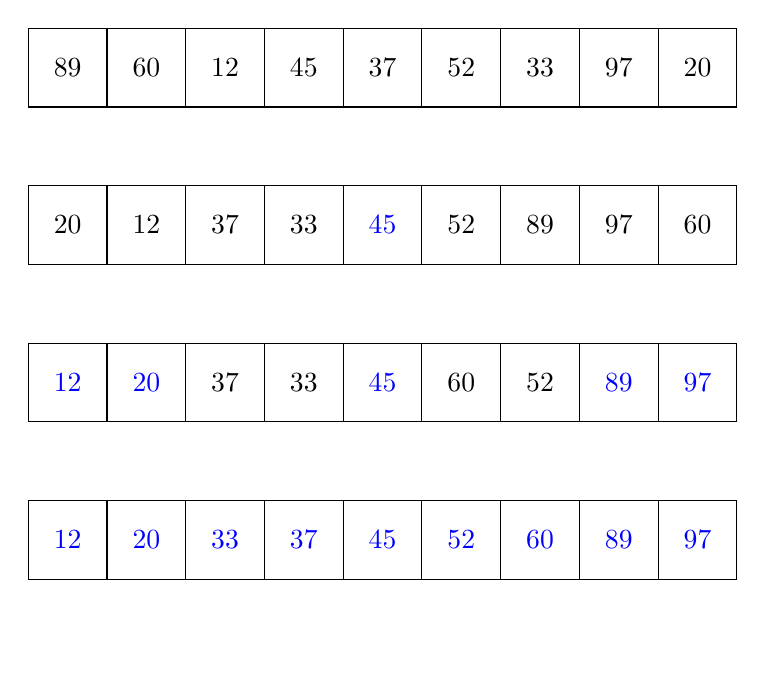
\begin{tikzpicture}
            \draw (0, 5) grid (9, 6);
            \draw[opacity=1] (0, 3) grid (9, 4);
            \draw[opacity=1] (0, 1) grid (9, 2);
            \draw[opacity=1] (0, -1) grid (9, 0);

            \draw[opacity=0] (0, -2) rectangle (1,-1);
            \draw[opacity=0,->] (2.5,0.5) node[anchor=north] { $p$ } -- (2.5,0.9);
            \draw[opacity=0,->] (6.5,0.5) node[anchor=north] { $p$ } -- (6.5,0.9);

            \node at (0.5, 5.5) { \textcolor{black}{$89$} };
            \node at (1.5, 5.5) { \textcolor{black}{$60$} };
            \node at (2.5, 5.5) { \textcolor{black}{$12$} };
            \node at (3.5, 5.5) { \textcolor{black}{$45$} };
            \node at (4.5, 5.5) { \textcolor{black}{$37$} };
            \node at (5.5, 5.5) { \textcolor{black}{$52$} };
            \node at (6.5, 5.5) { \textcolor{black}{$33$} };
            \node at (7.5, 5.5) { \textcolor{black}{$97$} };
            \node at (8.5, 5.5) { \textcolor{black}{$20$} };

            \node at (0.5, 3.5) { \textcolor{black}{$20$} };
            \node at (1.5, 3.5) { \textcolor{black}{$12$} };
            \node at (2.5, 3.5) { \textcolor{black}{$37$} };
            \node at (3.5, 3.5) { \textcolor{black}{$33$} };
            \node at (4.5, 3.5) { \textcolor{blue}{$45$} };
            \node at (5.5, 3.5) { \textcolor{black}{$52$} };
            \node at (6.5, 3.5) { \textcolor{black}{$89$} };
            \node at (7.5, 3.5) { \textcolor{black}{$97$} };
            \node at (8.5, 3.5) { \textcolor{black}{$60$} };

            \node at (0.5, 1.5) { \textcolor{blue}{$12$} };
            \node at (1.5, 1.5) { \textcolor{blue}{$20$} };
            \node at (2.5, 1.5) { \textcolor{black}{$37$} };
            \node at (3.5, 1.5) { \textcolor{black}{$33$} };
            \node at (4.5, 1.5) { \textcolor{blue}{$45$} };
            \node at (5.5, 1.5) { \textcolor{black}{$60$} };
            \node at (6.5, 1.5) { \textcolor{black}{$52$} };
            \node at (7.5, 1.5) { \textcolor{blue}{$89$} };
            \node at (8.5, 1.5) { \textcolor{blue}{$97$} };

            \node at (0.5, -0.5) { \textcolor{blue}{$12$} };
            \node at (1.5, -0.5) { \textcolor{blue}{$20$} };
            \node at (2.5, -0.5) { \textcolor{blue}{$33$} };
            \node at (3.5, -0.5) { \textcolor{blue}{$37$} };
            \node at (4.5, -0.5) { \textcolor{blue}{$45$} };
            \node at (5.5, -0.5) { \textcolor{blue}{$52$} };
            \node at (6.5, -0.5) { \textcolor{blue}{$60$} };
            \node at (7.5, -0.5) { \textcolor{blue}{$89$} };
            \node at (8.5, -0.5) { \textcolor{blue}{$97$} };

        \end{tikzpicture}

    \end{figure}

\end{frame}


\begin{frame}[fragile]{Implementação do {\it quicksort}}
    \inputsnippet{cpp}{27}{37}{codes/quicksort.cpp}
\end{frame}


